%# -*- coding: utf-8-unix -*-

\chapter{结合隐性特征的机票推荐算法}
\label{chap:latent}

我们在前几章中介绍了建立特征分布模型表达用户对机票的偏好。为用户建模的过程分为两步,首先从机票数据字段中抽取能反映机票主要内容的显性特征,再根据用户在每个特征内容上的选择分布进行用户建模。本章,我们结合机票的隐性特征建立用户偏好模型,并进行个性化机票推荐。

\section{用户出行性质对机票推荐准确率的影响}

我们将第三章中提出的用户特征分布模型进行上线部署并进行了一段时间的A/B测试对照实验。实验将用户随机分流,一部分用户(实验组)看到的候选机票列表是经过个性化推荐过后的搜索结果展示页。对于航线冷启动用户,我们在线上生产环境中采取了特征打分的原则并提供多样性推荐;其他用户(对照组)看到的是原版展示页。实验的主要观测指标是用户转化率,即订购机票的用户占浏览过机票用户总数的比例。A/B测试证实,实验组比对照组的转化率有所提升,但在周末和节假日时,实验组的转化率有所下降。我们通过分析发现,主要有两方面的原因。

\begin{figure}
 \centering
 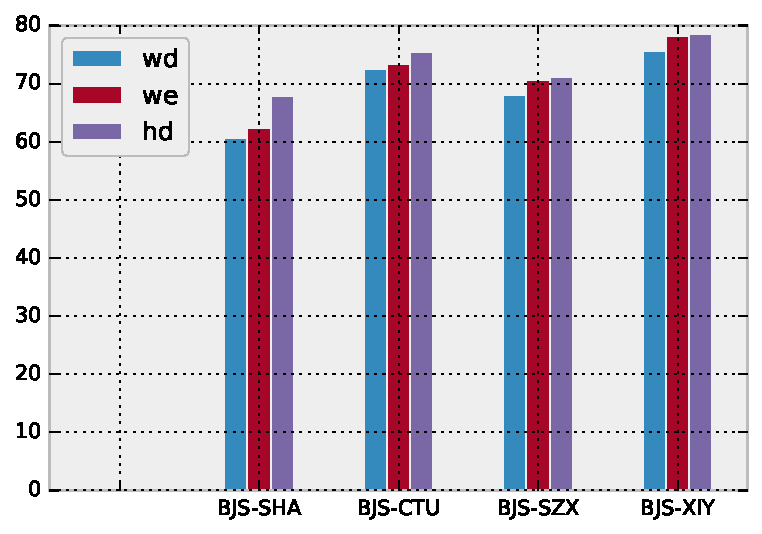
\includegraphics[width=0.6\linewidth]{04/1_inac_count.pdf}
 \bicaption[fig:inac_per]{冷启动用户占比}{不同起飞日期冷启动用户占比}{Fig}{Percentage of Inactive Users at Different Takeoff Date}
\end{figure}

图\ref{fig:inac_per}展示了四条航线在不同起飞日期航线冷启动用户占比。我们将起飞日期分为工作日(wd)、周末(we)和节假日(hd)。可以看到,不同航线上的冷启动用户比例总体有差距。北京-上海和北京-深圳的航线冷启动用户数量处于较低比例;北京-成都和北京-西安的航线冷启动用户数量处于较高比例。对每条航线而言,工作日的航线冷启动用户占比最低;周末和节假日的航线冷启动用户占比都较高,并且比例很接近。其中以北京-上海航线的工作日和节假日的冷启动用户比例差异最大。可以发现,非活跃用户比例差异的是第一个原因。在周末和节假日,航线非活跃用户比例增加,导致推荐效果的差异。第二个原因与用户行为变化相关。我们主要关注用户的出行性质。

用户的出行性质多种多样,如出差、参会、探亲、旅游等。总体来说可以分为商务性质和个人性质。对于出行性质是商务的乘客由于其行程安排及工作单位的差旅政策等因素,可能会更多地关注起飞时间、航空公司等特征,而对价格,舱位等特征关注较少;对于出行性质是个人的乘客,则更关注价格、退改签政策等特征。即使对于同一位用户,如果其出行性质不同,那么在购买机票时的关注点也会不同,从而产生用户行为的变化。用户的出行性质是一个无标签分类问题,它不能直接体现在订单数据中。因而我们无法对这个问题进行实验验证。但是我们可以通过直接对比推荐准确率,分析用户的行为是否产生变化。

\begin{figure}[!h]
 \centering
 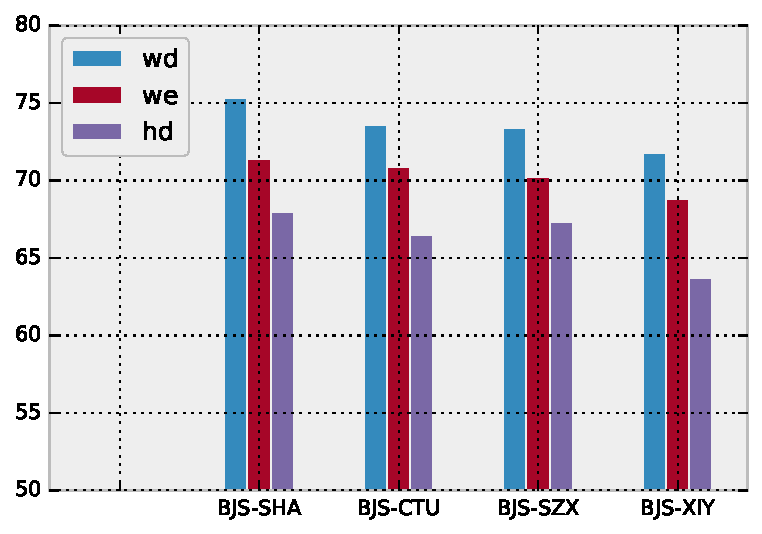
\includegraphics[width=0.6\linewidth]{04/2_wehd_rec.pdf}
 \bicaption[fig:at_rec]{分期机票推荐}{不同起飞日期机票推荐平均准确率}{Fig}{Mean Accuracy of Flight Recommendation at Different Takeoff Date}
\end{figure}

我们同样将测试订单按起飞日期分为工作日、周末和节假日三组。不同的是,我们只对各航线的活跃用户进行推荐实验。排除了不同起飞日期冷启动用户比例不同对推荐效果产生的影响。图\ref{fig:at_rec}是四条航线在不同起飞日期的机票推荐准确率。可以看出,在四条航线上,工作日的机票推荐准确率高于周末;而节假日的推荐效果最差。并且,工作日和周末的机票推荐准确率差异较小,而节假日的机票推荐准确率与前两类起飞日期的差异较大。

由此可以得出,用户行为在不同的起飞日期会产生一定的变化。前几章中以显性特征进行统计与分析所建立的用户特征分布模型虽然在一定程度上可以很好地概括用户的偏好习惯,也具有较强的解释性。但这种模型无法反映用户行为的变化。因此我们提出了结合隐性特征的用户偏好模型。在模型中,我们添加了起飞日期这一特征,旨在建立用户行为与起飞日期之间的关系。该特征的分为工作日、周末、节假日三个维度。

\section{问题建模及目标函数优化}

机票推荐属于隐式推荐,即用户不会对机票进行评分。在前几章介绍的推荐算法中,我们使用用户模型为候选机票列表中的每张机票都计算一个评分,按照这个评分为机票进行排序。并认为该用户对排序越靠前的机票具有越强的偏好。本质上相当于我们为用户和机票之间建立了一个效用函数。效用函数体系包括用户和物品两项,在我们的用户特征分布模型中,用户的模型就是用户项,而机票的特征内容向量就代表物品项。两者计算出的评分就是效用函数的值,函数值越大,代表用户对物品具有越强的偏好。

\begin{equation}
\label{eq:utility}
	V(u,i) = \phi_u^T * \theta_i
\end{equation}

\begin{equation}
\label{eq:phi_u}
	\phi_u = W_u * K_u
\end{equation}

\begin{equation}
\label{eq:theta_i}
	\theta_i = M_i * F_i
\end{equation}

\begin{table}[!hpb]
  \centering
  \bicaption[tab:lat_model]{参数介绍}{结合隐性特征的偏好模型}{Table}{Latent Factor Based Preference Model}
  \begin{tabular}{|c|c|} \hline 
V(U,I) & 用户U对机票I的偏好程度 \\ \hline
$\phi_u$ & 隐性空间上的用户偏好,维度 |W * 1| \\ \hline
$\theta_i$ & 隐性空间的机票特征,维度 |W * 1| \\ \hline
$W_u$ & 用户偏好转换矩阵,维度|W * K| \\ \hline
$K_u$ & 用户的显性特征偏好模型,增加起飞日期偏好,维度 |K * 1| \\ \hline
$M_i$ & 机票特征转换矩阵,维度 |W * F| \\ \hline
$F_i$ & 机票显性特征,增加起飞日期特征,维度 |F * 1| \\ \hline
  \end{tabular}
\end{table}

式\ref{eq:utility}代表效用函数,$\phi_u$代表用户的偏好,$\theta_i$代表物品的特征。在结合隐形特征模型中,我们将用户在显性空间上的特征分布模型$K_u$通过转换矩阵$W_u$转换到隐性空间;类似地,将物品在显性空间上的特征$F_i$通过转换矩阵$M_i$转换到隐性空间。我们将起飞日期作为特征,添加到$K_u$和$F_i$中。每个参数的含义及维度详细列在表\ref{tab:lat_model}中。

\begin{eqnarray}
\label{eq:pij}
    P(i,j) & = & P(V(u,i) > V(u,j)) \nonumber \\
	 & = &\frac{1}{1+e^{-(V(u,i) - V(u,j))}}
\end{eqnarray}

式\ref{eq:pij}中,$P(i,j)$代表用户对物品$i$比物品$j$有更强偏好的概率。我们为用户在两张机票上的偏好比较概率建立一个Sigmoid函数\parencite{jingfan1997novel}。如果我们假设用户选择的机票在候选机票列表中具有最强的偏好。则可以将用户实际选择的机票和任意一条候选机票构成一组成对(pair-wise)关系,并将式\ref{eq:pij}作为目标函数进行迭代学习。最终的学习效果是使得用户实际购买的机票有最大的效用值。该模型的目标函数如下:

\begin{equation}
\label{eq:cost}
  \arg\min_{W,M} : - \log P(i,j) + \frac{\lambda}{2} * (\sum_{i,j \in W}W_{i,j}^2 + \sum_{i,j \in M}M_{i,j}^2)
\end{equation}

我们的待估参数是$W$和$M$这两个转换矩阵。式\ref{eq:cost}中,为了简化训练过程,我们对$P(i,j)$取对数;同时加上正则项以防止过拟合。在参数训练步骤,我们使用梯度下降算法:

\begin{equation}
	W_u = W_u + \alpha(\frac{\partial \log P(i,j)}{W_u} - \lambda*W_u)
\end{equation}

\begin{equation}
	M_i = M_i + \alpha(\frac{\partial \log P(i,j)}{M_i} - \lambda*M_i)
\end{equation}

式中,$\alpha$代表学习速率。每次迭代过程分别就目标函数对参数$W_u$和$M_i$求梯度,并向负梯度方向进行迭代。为了确保用户实际选择的机票具有最大的效用,需要分别将所有候选机票与实际选择机票构建成对关系,并且用户的每一单训练订单都参入到训练过程中。这样会造成巨大的训练计算量。在实际实现中,我们从候选机票中随机抽取样本组成训练对。并且在训练每对样本时对参数矩阵进行更新。

此外,我们还提出了一种基于偏好排序的抽样训练策略。在基于用户特征分布模型的推荐中,已经可以获取重排序后的候选机票列表。因此我们可以只对排序在实际选择机票之前的候选机票进行抽样训练。这样的训练策略关注了显性用户模型无法捕获的用户行为波动变化和特征间联系对推荐效果的影响,强化了学习效率。

\section{结合隐性特征的机票个性化推荐}

在前面的章节中,我们主要关注用户在不同出发日期的行为变化,并尝试使用转换矩阵将用户和机票在显性空间上的特征分布与内容都映射到隐形空间,以此捕捉用户的行为变化和显性特征间的联系。并基于用户的训练订单,使用随机抽样的梯度下降法对转换矩阵参数进行训练。得到训练后的转换矩阵后,我们可以计算用户对每条候选机票的效用函数$V(u,i)$,并根据效用函数对机票进行排序。在进行机票推荐时,我们可以将根据显性用户模型和隐性用户偏好模型的排序结果综合起来,作为最终推荐结果。

\begin{equation}
\label{eq:mix_rat}
	R(I) = R(P_u^T * F_I) + R(\phi_u^T * \theta_I)
\end{equation}

式\ref{eq:mix_rat}中,第一项代表了根据显性用户模型得到的排序结果,第二项代表根据隐性偏好模型的排序结果。我们最终根据每张机票的总体排位$R(I)$为用户进行推荐。

\begin{algorithm}
\caption{结合隐性特征的机票推荐}
\label{algo:lat_rec}
\begin{algorithmic}[1]
\Require
\Statex 用户历史订单 $O$
\Statex 机票特征集合 $F$
\Statex 搜索结果列表 $C$

\Ensure 
\Statex 排序后的机票列表 $R$

\State $W_u \gets \mathbf{0}$;
\State $M_i \gets \mathbf{0}$;


\For { $o \in O$}
\State $C_o \gets getSearchResult(o)$;
\For { $t_o \in C_o.sample()$}

\State $W_u = W_u + \alpha(\frac{\partial \log P(o,t_o)}{W_u} - \lambda*W_u)$;
\State $M_i = M_i + \alpha(\frac{\partial \log P(o,t_o)}{M_i} - \lambda*M_i)$;
\EndFor
\State If reach iteration limit, break
\EndFor

\For { $t \in C$}
\State $R_t = R(P_u^T * F_t) + R(\phi_u^T * \theta_t)$
\State Append $R_t$ to R
\EndFor 
\State Sort $R$ by ascending;
\State \Return $R$
\end{algorithmic}
\end{algorithm}

算法\ref{algo:lat_rec}展示了结合隐性特征的机票推荐算法的流程。在模型训练过程中,我们使用用户历史订单作为训练集。对于每一条训练数据,我们需要获取当时的模拟搜索结果,其方法与在第三章进行推荐实验时相同,以航班、起飞日期和舱位为筛选条件,从全体订单数据中检索。每次训练,我们在搜索结果中进行取样,与该条订单数据构成一组成对关系,并更新参数。当到达迭代停止条件后停止训练,这里的迭代停止条件包括到达迭代次数、结果收敛以及训练订单的效用达到最大值。

在机票推荐过程中,我们对候选机票列表中的每张机票的显性用户模型排序和隐性用户模型排序综合起来,得到最终的推荐列表。算法的计算复杂度是$O(WN)$,其中$W$是隐形空间的特征数量,$N$是迭代次数上限。可以认为,该算法与隐形特征数量呈线性关系。


\section{实验结果分析}

本节我们对结合隐性特征的机票推荐进行实验及分析。我们将介绍实验数据集、评价指标以及机票推荐结果。

\subsection{实验数据集与评价指标}
在实验中,我们选取北京到上海,北京到成都,北京到深圳,北京到西安四条航线的活跃用户作为测试用户。我们将测试订单按起飞日期分成工作日、周末、节假日三类。研究结合隐性特征的模型是否能够适应用户在不同起飞日期的行为变化。

本章我们仍使用第三章实验评价指标,式\ref{eq:a-rec}对每条机票推荐准确率进行评价,
式\ref{eq:ma}对为所有用户的机票推荐平均准确率进行评价。

\subsection{机票推荐准确率}

\begin{figure}
 \centering
 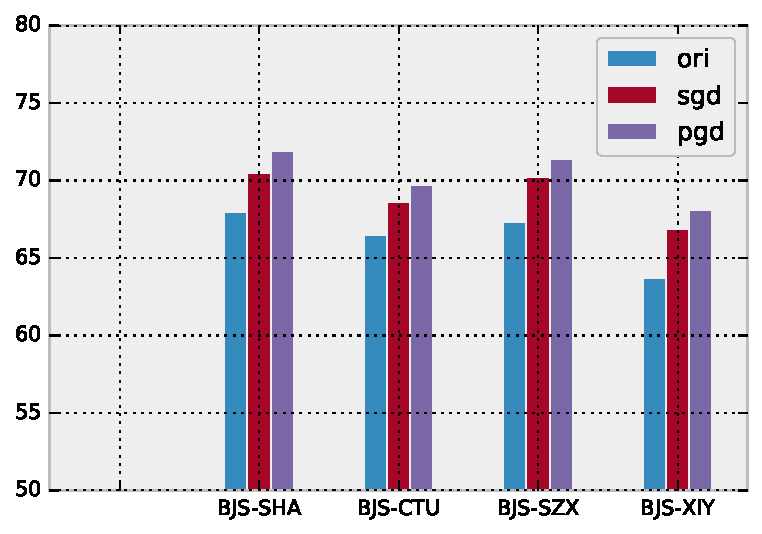
\includegraphics[width=0.6\linewidth]{04/3_lat_rec.pdf}
 \bicaption[fig:la_hd_rec]{节假日机票推荐}{结合隐形特征模型在节假日的机票推荐准确率}{Fig}{Mean Accuracy for Latent Factor Combined Flight Recommendation at Holidays}
\end{figure}

图\ref{fig:la_hd_rec}展示了四条航线在节假日的推荐结果。包括显性用户模型(ori)、随机样本模型(sgd)、偏好排序样本模型(pgd)。如前文所述,sgd和pgd的区别是,前者使用随机抽样成对样本进行模型训练;后者使用根据显性偏好排序的成对样本进行模型训练。可以看出,结合隐性特征的机票推荐准确率比仅使用显性用户模型有所提升。而使用基于偏好排序样本的训练模型对机票推荐准确率相较随机样本模型的推荐准确率有少量提升。可以证明,结合隐性特征的用户模型可以反映出用户在节假日的行为变化,也能够一定程度上挖掘到机票显性特征之间的关联。


\begin{table}[!h]
  \centering
  \bicaption[tab:sha_all_day]{推荐效果}{北京-上海航线不同起飞日期的机票推荐准确率}{Table}{Mean Accuracy of Flight Recommendation at Different Takeoff Date}
  \begin{tabular}{|c|c|c|c|} \hline 
模型 & 节假日 & 周末 & 工作日 \\ \hline
显性模型 & 68.0\% & 71.4\% & 75.3\% \\ \hline
随机样本模型 & 70.5\% & 72.8\% & 75.7\% \\ \hline
偏好排序样本模型 & 71.9\% & 73.4\% & 76.2\% \\ \hline
  \end{tabular}
\end{table}

表\ref{tab:sha_all_day}展示了北京-上海航线在工作日、周末、节假日三类起飞时间的个性化机票推荐准确率。可以看到,在周末和工作日,结合隐性特征的用户模型对机票推荐准确率仍有提升,并且使用偏好排序样本模型的提升高于随即样本。但在工作日,结合隐性模型的机票推荐效果提升较少。

\section{本章小结}

本章我们研究了用户在不同起飞日期的行为变化对个性化机票推荐准确率带来的影响。我们将测试订单进行分组,并使用实验验证了节假日的机票推荐准确率低于周末及工作日。为了使模型能够反映用户的行为变化,我们为机票的显性内容增加了起飞时间类型这一特征,并建立了转换矩阵将用户特征分布模型和机票内容都映射到隐性空间。基于用户对实际选择的订单具有更高效用的假设,定义了基于成对模型的目标优化函数,并使用梯度下降法进行参数推导。在取样构建成对关系的过程中,我们提出了基于显性偏好排序的抽样方法。实验结果证实,结合隐性特征的用户模型可以反映出用户在节假日的行为变化以及显性特征之间的联系,能够提升个性化机票推荐效果。